% !TeX spellcheck = sl_SI
% vim: set spell spelllang=sl:
% za preverjanje črkovanja, če se uporablja Texstudio ali vim
\documentclass[12pt,a4paper,twoside]{article}
\usepackage[utf8]{inputenc}  % pravilno razpoznavanje unicode znakov

% NASLEDNJE UKAZE USTREZNO POPRAVI
\newcommand{\program}{IŠRM} % ime studijskega programa
\newcommand{\imeavtorja}{Klemen Kobau} % ime avtorja
\newcommand{\imementorja}{izr.~prof.~dr. Mojca Ciglarič} % akademski naziv in ime mentorja, uporabi poln naziv, prof.~dr.~, doc.~dr., ali izr.~prof.~dr.
\newcommand{\imesomentorja}{as. Miha Grohar} % akademski naziv in ime somentorja, če ga imate
\newcommand{\naslovdela}{Avtomatizacija namestitve aplikacije “Big Data” v privatni in javni oblak}
\newcommand{\letnica}{2022} % letnica magistriranja
\newcommand{\opis}{Delo obravnava integracijo po ω-kompleksih, njene lastnosti in posplošitve
na Levy-jeve topološke prostore.}  % Opis dela v eni povedi. Ne sme vsebovati matematičnih simbolov v $ $.
\newcommand{\kljucnebesede}{integracija\sep kompleks} % ključne besede, ločene z \sep, da se PDF metapodatki prav procesirajo
\newcommand{\keywords}{integration\sep complex} % ključne besede v angleščini
\newcommand{\organization}{Univerza v Ljubljani, Fakulteta za matematiko in fiziko} % fakulteta
\newcommand{\literatura}{literatura}  % pot do datoteke z literaturo (brez .bib končnice)
\newcommand{\sep}{, }  % separator med ključnimi besedami v besedilu
% KONEC PODATKOV

\usepackage{bibentry}         % za navajanje literature v programu dela s celim imenom
\nobibliography{\literatura}
\newcommand{\plancite}[1]{\item[\cite{#1}] \bibentry{#1}} % citiranje v programu dela

% OBSOLETE \usepackage{filecontents}  % za pisanje datoteke s PDF metapodatki
\usepackage{silence} \WarningFilter{latex}{Overwriting file}  % odstrani annoying warning o obstoju datoteke
% datoteka s PDF metapodatki, zgenerira se kot magisterij.xmpdata
\begin{filecontents*}{\jobname.xmpdata}
  \Title{\naslovdela}
  \Author{\imeavtorja}
  \Keywords{\kljucnebesede}
  \Subject{matematika}
  \Org{\organization}
\end{filecontents*}

\usepackage[a-1b]{pdfx}  % zgenerira PDF v tem PDF/A-1b formatu, kot zahteva knjižnica
\hypersetup{bookmarksopen, bookmarksdepth=3, colorlinks=true,
  linkcolor=black, anchorcolor=black, citecolor=black, filecolor=black,
  menucolor=black, runcolor=black, urlcolor=black, pdfencoding=auto,
  breaklinks=true, psdextra}

\usepackage[slovene]{babel}  % slovenščina
\usepackage[autostyle=false, style=german]{csquotes}
\usepackage[T1]{fontenc}     % naprednejše kodiranje fonta
\usepackage{amsmath,amssymb,amsfonts,amsthm} % matematični paketi
\usepackage{graphicx}     % za slike
\graphicspath{ {./images/} }
\usepackage{emptypage}    % prazne strani so neoštevilčene, ampak so štete
\usepackage{units}        % fizikalne enote kot \unit[12]{kg} s polovico nedeljivega presledka, glej primer v kodi
%\usepackage{makeidx}      % za stvarno kazalo, lahko zakomentiraš, če ne rabiš
%\makeindex                % za stvarno kazalo, lahko zakomentiraš, če ne rabiš
% oblika strani
\usepackage[
  top=3cm,
  bottom=3cm,
  inner=3.5cm,      % margini za dvostransko tiskanje
  outer=2.5cm,
  footskip=40pt     % pozicija številke strani
]{geometry}
\usepackage{floatrow}

% VEČ ZANIMIVIH PAKETOV
% \usepackage{array}      % več možnosti za tabele
% \usepackage[list=true,listformat=simple]{subcaption}  % več kot ena slika na figure, omogoči slika 1a, slika 1b
% \usepackage[all]{xy}    % diagrami
\usepackage{doi}        % za clickable DOI entrye v bibliografiji
% \usepackage{enumerate}     % več možnosti za sezname

% Za pisanje psevdokode
% \usepackage{algpseudocode}  % za psevdokodo
% \usepackage{algorithm}
% \floatname{algorithm}{Algoritem}
% \renewcommand{\listalgorithmname}{Kazalo algoritmov}

% DRUGI TVOJI PAKETI:
% tukaj
\usepackage[nocompress]{cite}
\usepackage{xargs}
\usepackage[colorinlistoftodos,prependcaption,textsize=tiny]{todonotes}
\newcommandx{\unsure}[2][1=]{\todo[linecolor=red,backgroundcolor=red!25,bordercolor=red,#1]{#2}}
\newcommandx{\info}[2][1=]{\todo[linecolor=blue,backgroundcolor=blue!25,bordercolor=blue,#1]{#2}}
\newcommandx{\change}[2][1=]{\todo[linecolor=green,backgroundcolor=green!25,bordercolor=green,#1]{#2}}
\newcommandx{\improvement}[2][1=]{\todo[linecolor=orange,backgroundcolor=orange!25,bordercolor=orange,#1]{#2}}

\usepackage[
    left = \glqq{},% 
    right = \grqq{},% 
    leftsub = \glq{},% 
    rightsub = \grq{} %
]{dirtytalk}

\usepackage{listings}
\renewcommand{\lstlistingname}{Primer}

\usepackage{appendix}
\renewcommand{\appendixname}{Priloga}
\renewcommand{\appendixtocname}{Priloge}
\renewcommand{\appendixpagename}{Priloge}

\usepackage{tabularx}
\newcolumntype{L}{X}
\newcolumntype{S}{>{\hsize=.5\hsize}X}
\newcolumntype{Q}{>{\hsize=.1\hsize}X}

\setlength{\overfullrule}{50pt} % označi predlogo vrstico
\pagestyle{plain}               % samo številka strani na dnu, nobene glave / noge

\newcounter{phaseCounter}
\setcounter{phaseCounter}{1}
\newcommand{\phase}[1]{\subsection{Faza \arabic{phaseCounter}: #1} \stepcounter{phaseCounter}}

\newcommand{\tablegraphics}[1]{\vspace{1pt plus 1pt minus 0pt} \includegraphics[scale = 0.3]{#1}}

% \DeclareMathOperator{\tr}{tr}  % morda potrebuješ operator za sled ali kaj drugega?

% bold matematika znotraj \textbf{ }, tudi v naslovih, kot \omega spodaj
\makeatletter \g@addto@macro\bfseries{\boldmath} \makeatother

% Poimenuj kazalo slik kot ``Kazalo slik'' in ne ``Slike''
\addto\captionsslovene{
  \renewcommand{\listfigurename}{Kazalo slik}%
}

% če želiš, da se poglavja začnejo na lihih straneh zgoraj
%\let\oldsection\section
%\def\section{\cleardoublepage\oldsection}

%%%%%%%%%%%%%%%%%%%%%%%%%%%%%%%%%%%%%%%%%%
%%%%%%           DOCUMENT           %%%%%%
%%%%%%%%%%%%%%%%%%%%%%%%%%%%%%%%%%%%%%%%%%

\begin{document}

\pagenumbering{roman} % začnemo z rimskimi številkami
\thispagestyle{empty} % ampak na prvi strani ni številke

\noindent{\large
UNIVERZA V LJUBLJANI\\[1mm]
FAKULTETA ZA MATEMATIKO IN FIZIKO\\[5mm]

\noindent UNIVERZA V LJUBLJANI\\[1mm]
FAKULTETA ZA RAČUNALNIŠTVO IN INFORMATIKO\\[5mm]
\program\ -- 2.~stopnja}
% ustrezno dopolni za IŠRM
\vfill

\begin{center}
  \large
  \imeavtorja\\[3mm]
  \Large
  \textbf{\MakeUppercase{\naslovdela}}\\[10mm]
  \large
  Magistrsko delo \\[1cm]
  Mentorica: \imementorja \\[2mm] % ustrezno popravi spol
  Somentor: \imesomentorja   % dodaj, če potrebno
\end{center}
\vfill

\noindent{\large Ljubljana, \letnica}

\cleardoublepage

%% sem pride IZJAVA O AVTORSTVU  -- SE NATISNE V VIS

% zahvala
\pdfbookmark[1]{Zahvala}{zahvala} %
\section*{Zahvala}
Neobvezno.
Zahvaljujem se \dots
% end zahvala -- izbriši vse med zahvala in end zahvala, če je ne rabiš

\cleardoublepage

\pdfbookmark[1]{\contentsname}{kazalo-vsebine}
\tableofcontents

% list of figures
% \cleardoublepage
% \pdfbookmark[1]{\listfigurename}{kazalo-slik}
% \listoffigures
% end list of figures

\cleardoublepage

\section*{Seznam uporabljenih kratic in simbolov}

\noindent\begin{tabular}{p{0.1\textwidth} p{.35\textwidth} p{.4\textwidth}}
  {\bf kratica} & {\bf Daljše} & {\bf Razlaga} \\ \hline
  SQL & structured query language & strukturiran povpraševalni jezik \\
  NoSQL & not only SQL &  vrsta podatkovne baze, ki ni relacijska \\
  HDFS & Hadoop Distributed File System & Hadoop razpršen podatkovni sistem \\
  PaaS & Platform as a service & Platforma kot storitev \\
  HA & High Availability & Visoka dosegljivost \\
\end{tabular}

\section*{Slovarček}
\noindent\begin{tabular}{p{0.15\textwidth} p{.75\textwidth}}
  {\bf Termin} & {\bf Razlaga} \\ \hline
  Hadoop & Apache Hadoop je ogrodje za razpršeno 
  shranjevanje, procesiranje in analizo podatkov~\cite{tech_hadoop} \\
\end{tabular}


\cleardoublepage

\section*{Program dela}
\addcontentsline{toc}{section}{Program dela} % dodajmo v kazalo

\section*{Osnovna literatura}

\vspace{2cm}
\hspace*{\fill} Podpis mentorja: \phantom{prostor za podpis}

\vspace{2cm}
\hspace*{\fill} Podpis somentorja: \phantom{prostor za podpis}

\cleardoublepage
\pdfbookmark[1]{Povzetek}{abstract}

\begin{center}
\textbf{\naslovdela} \\[3mm]
\textsc{Povzetek} \\[2mm]
\end{center}
Tukaj napišemo povzetek vsebine. Sem sodi razlaga vsebine in ne opis tega, kako je delo
organizirano.

\vfill
\begin{center}
\textbf{English translation of the title} \\[3mm] % prevod slovenskega naslova dela
\textsc{Abstract}\\[2mm]
\end{center}

An abstract of the work is written here. This includes a short description of
the content and not the structure of your work.

\vfill\noindent
\textbf{Math.~Subj.~Class.~(2010):} oznake kot 74B05, 65N99, na voljo so na naslovu
\url{http://www.ams.org/msc/msc2010.html} \\[1mm]
\textbf{Ključne besede:} \kljucnebesede \\[1mm]
\textbf{Keywords:} \keywords

\cleardoublepage

\setcounter{page}{1}    % od sedaj naprej začni zopet z 1
\pagenumbering{arabic}  % in z arabskimi številkami

% CONTENT

\section{Uvod}

Informacijski sistemi, ki ji jih vsakodnevno uporablja sodobna družba, 
generirajo velike količine podatkov. 
Podatke generirajo uporabniki in aplikacije ...same. Ker je shranjevanje in 
obdelava velike količne podatkov podjetjem dostopnejša kot je bila nekoč, 
podjetja le te zkoriščajo za različne namene, od izboljšanja poslovnih strategij, 
dviga dodane vrednosti, segmentacije in profiliranja kupcev, 
do izboljšanja delovanja samih informacijskih sistemov in preprečevanja napak.
Za obdelavo velikih količin podatkov se je razvila računalniška smer, 
\textit{Podatkovne vede}, ki se ukvarja z analizo
in obvladovanjem teh podatkov.
Z \enquote{veliko količino} mislimo količine, ki segajo v terabite ali petabite 
in so generirane v sekundnih intervalih~\cite{toward_scalable_systems_big_data_analytics}.
Tradicionalne metode niso kos takim podatkovnim tokom, zato za obdelavo velike količine podatkov, 
predvsem v realnem času, 
potrebujemo specializirane tehnologije.
Takšni sistemi za obvladovanje kompleksnih podatkovnih tokov so ponavadi sestavljeni iz 
različnih komponent in modulov in 
s tem zelo zahtevni za postavitev in obvladovanje. 
Potrebnega je veliko specializiranega računalniškega predznanja, 
da se postavi ustrezna računalniška arhitektura, 
ki na učinkovit in hiter način podatke obravnava. 
Hkrati moramo skrbeti, da je delovanje takšnega sistema čimbolj zanesljivo in 
da pride do čim manj izgube podatkov.
Zaradi tega moramo razviti načine samodejnega popravljanja sistema v primerih izpadov.
Ob povečanju uporabe aplikacije in s 
tem pretoka podatkov si ne smemo privoščiti izpada delovanja sistema, 
zato si želimo, da se zna sistem samodejno prilagajati potrebam.

Ker ima danes vse več podjetij potrebo po uporabi lastnih Big Data aplikacij, 
v magistrski nalogi nalogi predstavimo metodologijo in nekaj konceptov,
katere potrebujemo kot ogrodje za postavitev poljubne Big Data aplikacije.
Podjetja lastne Big Data aplikacije najpogosteje postavljajo v računalniški oblak. 
Med vsemi lastnostmi je zaupnost podatkov ključna in 
odloča med postavitvijo Big data aplikacije v javnem (public cloud) ali privatnem oblaku, 
ki je lahko postavljen na lastni (on-prem) ali tuji infrastrukturi (off-prem).
Zato se v magisterski nalogi osredotočamo na najpogostejša načina namestitve,
v javnem ali privatnem oblaku. 
Primer je narejen na rešitvi Gamayun, ki je v lasti podjetja Medius, 
ampak naša metodologija ni vezana na to rešitev.

\subsection{Cilji in prispevki}
\subsection{Struktura magistrske naloge}

\section{Big data}

Definicija Big data še ni ustaljena.
Članek~\cite{toward_scalable_systems_big_data_analytics} predstavi 3 definicije.

\paragraph{Definicija preko lastnosti}
Big data aplikacije obdelujejo podatke z naslednjimi lastnostmi, katerimi se
skupno reče 4V, po angleških besedah za lastnosti.
Članek~\cite{modeling_requirements_big_data} navede tu še nekaj razlogov za izbrane 
lastnosti\footnote{Podatki so iz leta 2013, številke so se samo še povečale.}.

\begin{itemize} \label{list:four_v}
    \item Volumen podatkov (\emph{Volume}) -- Aplikacija uporablja velike količine podatkov (več terabajtov, petabajtov, zetabitov)
    \begin{itemize}
        \item Članek~\cite{modeling_requirements_big_data} napoveduje, da bo do leta 2020 generiranih 40 zetabitov podatkov 
        \footnote{Vir~\cite{big_data_amount_statista} to številko poveča na 64 zetabitov}, kar je 300 kratno povečanje od leta 2005
        \item 6 od 7 biljonov ljudi ima mobilni telefon
        \item Večina podjetij v ZDA ima vsaj 100 terabitov shranjenih podatkov
    \end{itemize}

    \item Hitrost podatkovnih tokov (\emph{Velocity}) -- Podatki so generirani v realnem času, ali skoraj v realnem času
    \begin{itemize}
        \item Newyorška borza shrani 1 terabit podatkov med vsako trgovsko sejo
        \item Moderni avtomobili imajo skoraj 100 senzorjev
    \end{itemize}
    
    \item Raznolikost podatkov (\emph{Variety}) -- podatkovni modeli so manj strokturirani, imamo več virov podatkov
    \begin{itemize}
        \item Od leta 2011 je bila ocena velikosti podatkov okoli 150 Exabitov
        \item Uporabniki YouTube pogledajo več kot 4 miljarde ur videoposnetkov vsak mesec
        \item 400 miljonov tweetov se pošlje vsak dan 
    \end{itemize}

    \item Zaupanje v podatke (\emph{Veracity}) -- podatki so lahko napačni, napake v podatkih.
    \begin{itemize}
        \item 1 izmed 3 vodilnih podjetij ne zaupa podatkom, katere uporabijo za odločitve 
    \end{itemize}
\end{itemize}

\paragraph{Definicija preko primerjave}
Big data pomeni delo s količino podatkov, ki jo tradicionalne baze ne podpirajo.

\paragraph{Definicija preko arhitekture}
Big data pomeni delo s podatki, kjer njihova količina preprečuje uporabo
tradicionalnih baz in potrebujemo precejšnje horizontalno skaliranje.

\bigskip

\noindent Big data nima ustaljene definicije, ampak s prej napisanimi si lahko pomagamo pri razumevanju razlik
pri delu z big data in tradicionalnim delom s podatki.

\subsection{Primerjava s tradicionalnimi podatki}

Članek~\cite{toward_scalable_systems_big_data_analytics} primerja delo s tradicionalnimi podatki in z big data.
Iz razlik med vrstama lažje razumemo zakaj tradicionalne metode za obdelavo podatkov niso primerne za obdelavo big data podatkov.

\begin{table}[H]
\centering
\begin{tabular}{l l l} 
& Tradicionalni & Big Data \\
\hline
Volumen & GB & se povečuje (TB, PB, EB) \\
Hitrost generiranja & vsako uro, dan & hitreje kot tradicionalni \\
Struktura & strukturirani & delno ali nestrukturirani \\
Viri & centralizirani & razpršeni \\
Integriteta & enostavna & težka \\
Shramba & relacijska & HDFS ali NoSQL \\
Dostop & interaktiven & v sklopih ali v realnem času
\end{tabular}
\caption{Primerjava podatkov v big data in v navadnih aplikacijah. Tabela je prevedena iz~\cite{toward_scalable_systems_big_data_analytics}.}
\label{table:big-data-vs-normal}
\end{table}

\subsection{Izzivi in priložnosti Big Data}

\todo{Napiši kaj o izzivih in priložnostih. O tem imam nek članek.}

\subsection{Primeri big data aplikacij}
Avtorji~\cite{vehicle_networks} predstavijo način izboljšave prenosa podatkov med vozili.
Uporabijo povezave naprava-naprava, kjer skupine avtomobilov skupaj tvorijo center za oddajo podatkov, ki
so zelo zahtevani in je zahtevkov preveč za eno samo vozilo.
Soočajo se z velikimi količinami podatkov, kjer kjer lahko deli arhitekture nenadoma odpovejo.
Podatki so nestrukturirani in generirani v realnem času.

Članek~\cite{a_big_data_analytics_based_methodology} govori o uporabi big data za sprejemanje strateških odločitev
pri trgovanju.
Avtorji nadgradijo CRISP-DM\todo{dodaj v slovarček, opiši, citiraj} metodologijo.
Izboljšano metodologijo nato uporabijo za analizo trgov.

Avtorji~\cite{scalable_framework_for_provisioning_large_scale_iot_deployments} predstavijo orodje LEONORE,
ki omogoča elastično postavljanje ogrodja za aplikacije na meji\todo{edge computing, dodaj prevod}.
Soočijo se s težavo postavljanja procesorsko zahtevnih aplikacij na napravah z malo procesorske moči.
\improvement{Dopolni}

Več primerov big data aplikacij na različnih področjih si lahko preberete v~\cite{big_data_analytics_societal_impact}.

\todo{Dodaj več primerov}

\section{Big data arhitektura}

\subsection{Arhitektura aplikacij}
Aplikacijska arhitektura opisuje načine in tehnike, ki so uporabljene pri zasnovi in gradnji aplikacije.
Arhitektura nam olajša načrtovanje poteka razvoja in nam poda dobre prakse za grajenje aplikacij~\cite{application_architecture_def}.
Skozi čas se je razvilo več tipov arhitektur, spodaj opišemo samo nekatere.

\paragraph{Monolitna arhitektura}
Vse funkcionalnosti so združene skupaj v eni aplikaciji.
Za vsako posodobitev moramo ponovno izdati celo aplikacijo in različne funkcionalnosti so močno povezane.

\paragraph{Mikrostoritve}
Aplikacije razbijemo na najmanjše dele, ki so neodvisni en od drugega.
Vsako mikrostoritev lahko posodobimo neodvisno, funkcionalnosti so neodvisne ena od druge.

\paragraph{Arhitektura vodena preko dogodkov}
Imamo proizvajalce in porabnike dogodkov.
Proizvajalci se ne zavedajo porabnikov, kar pomeni večjo neodvisnost.
Z dodajanjem novih proizvajalcev in porabnikov lahko arhitekturo enostavno skaliramo.

\subsection{Izzivi big data arhitekture}
\todo{Primerjava s tradicionalno arhitekturo}
Avtorji v članku~\cite{provisioning_big_data_micro_cloud} predstavijo težave dinamičnega priskrbovanja big data aplikacij.
Predstavijo naslednje izzive.

\paragraph{Konfiguracija in postavljanje}
Tehnologije, ki so uporabljene v arhitekturi so ponavadi kompleksne in imajo veliko parametrov.
Za njihovo nastavitev potrebujemo zaposlene z znanjem teh tehnologij in že majhna napaka lahko pomeni slabše
delovanje.

\paragraph{Elastičnost}
Obremenitve aplikacije se lahko hitro spreminjajo.
Želimo jih hitro zaznati in se jim prilagoditi, saj s tem prihranimo denar, ali pa preprečimo počasno delovanje
ob nenadnih poskokih zahtevnosti.

\paragraph{Visoka razpoložljivost}\label{par:high_availability}
Napake so v aplikacijah pričakovane, saj lahko pride do napak v strojni opremi, napak v samih aplikacijah ali
napak pri komunikaciji med aplikacijami.
Napakam se moramo znati prilagoditi in zmanjšati čas, ko je naša aplikacija nedosegljiva.
Preprečiti moramo izgube ali nedosegljivosti podatkov.
Članek~\cite{ha_computer_systems} opiše visoko dosegljivost in načine, kako jo lahko dosežemo.
Grobo, visoka dosegljivost pomeni, da mora biti naša aplikacija dostopna 99.999\% časa, kar pomeni, da je lahko
nedostopna 5 minut na leto.

\paragraph{Sobivanje aplikacij}
\todo{Dodaj prevode: multy-tenancy}
Aplikacije različnih strank kdaj bivajo v istem okolju.
Aplikacije morajo biti med sabo izolirane in aplikacija ene stranke ne sme povzročiti izpada aplikacije 
neke druge stranke.

\paragraph{Verzioniranje in podpiranje različnih verzij}
Želimo imeti vodenje verzij aplikacije in različnih tehnologij, ki so uporabljene za podporo aplikacije.
V nekaterih primerih moramo hkrati ponujati več različnih verzij iste aplikacije 
ali njihovih podpornih komponent saj ni nujno, da vsi odjemalski sistemi podpirajo 
ali so prilagojeni za delovanje na najnovejših verzijah podpornih tehnologijah.

\paragraph{Ostali izzivi}
Varnost in upoštevanje licenc, ki pa nista značilni samo za big data aplikacije.

\subsection{Arhitekturi Kappa in Lambda}

Arhitekture Big Data so raznolike,
ampak okvirno jih lahko uvrstimo v dva razreda: Kappa ali Lambda arhitekturo~\cite{kappa_lambda}.
Lambda arhitektura vsebuje storitve za procesiranje podatkovnih tokov
in za procesiranje paketov, medtem ko Kappa vsebuje samo storitve za
procesiranje tokov in delo s paketi obravnava kot tokove z zakasnitvijo.

Kappa in Lambda predstavljata dva načina razmišljanja in sicer posploševanje in
specializacija.
Kappa je posplošena, kar pomeni da nam ni treba pisati konfiguracij
za storitve za delo s paketi in ni usklajevanja med storitvami,
ampak zaradi tega je delovanje počasnejše, kot če bi imeli orodje,
ki je specializirano za delo s paketi.
Pri Lambdi je problem ravno obraten, imamo pravo orodje,
ampak moramo usklajevati konfiguracijo med storitvami za tokove in za pakete.

\subsection{Primeri big data arhitektur}

V tem odseku predstavimo nekaj arhitektur znanih podjetij~\cite{reference_architecture_classification_technologies}.
Na koncu predstavimo referenčno arhitekturo,
ki je povzeta iz članka~\cite{reference_architecture_classification_technologies} in je
podobna referenčni arhiteturi iz članka~\cite{reference_architecture_bd}.
Arhitektura Facebooka je predstavljena v sliki~\ref{fig:arch-facebook}, arhitektura Twitterja pa v sliki~\ref{fig:arch-twitter}.

\begin{figure}[H]
    \centering
    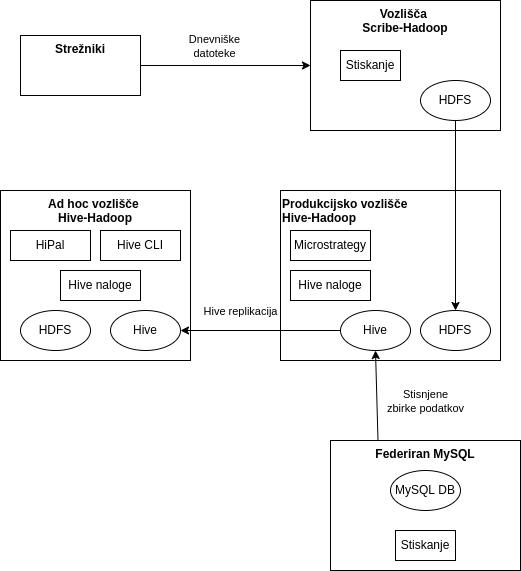
\includegraphics[width=0.6\textwidth]{img/arhitektura/podjetja/facebook.png}
    \caption{Arhitektura za analizo podatkov pri Facebook~\cite{reference_architecture_classification_technologies}.}
    \label{fig:arch-facebook}
\end{figure}

\begin{figure}[H]
    \centering
    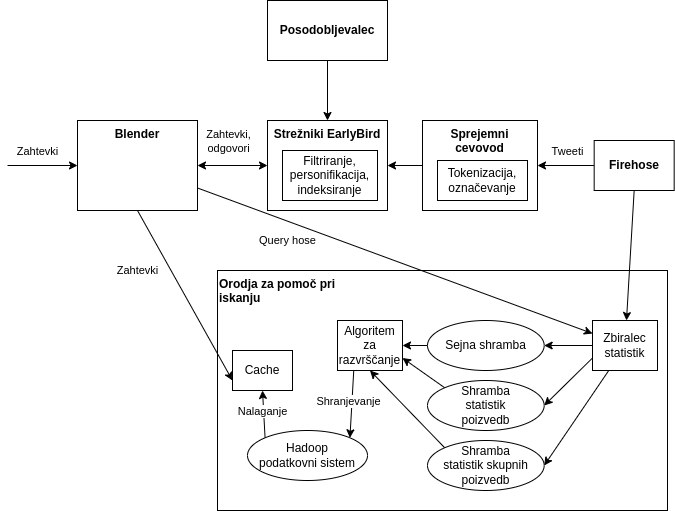
\includegraphics[width=0.8\textwidth]{img/arhitektura/podjetja/twitter.png}
    \caption{Arhitektura za analizo podatkov pri Twitterju~\cite{reference_architecture_classification_technologies}.}
    \label{fig:arch-twitter}
\end{figure}

\noindent Iz več primerov arhitektur, avtorji članka~\cite{reference_architecture_classification_technologies}
ustvarijo referenčno arhitekturo za Big Data, ki je predstavljena v sliki~\ref{fig:arch-ref-article}.

\begin{figure}[H]
    \centering
    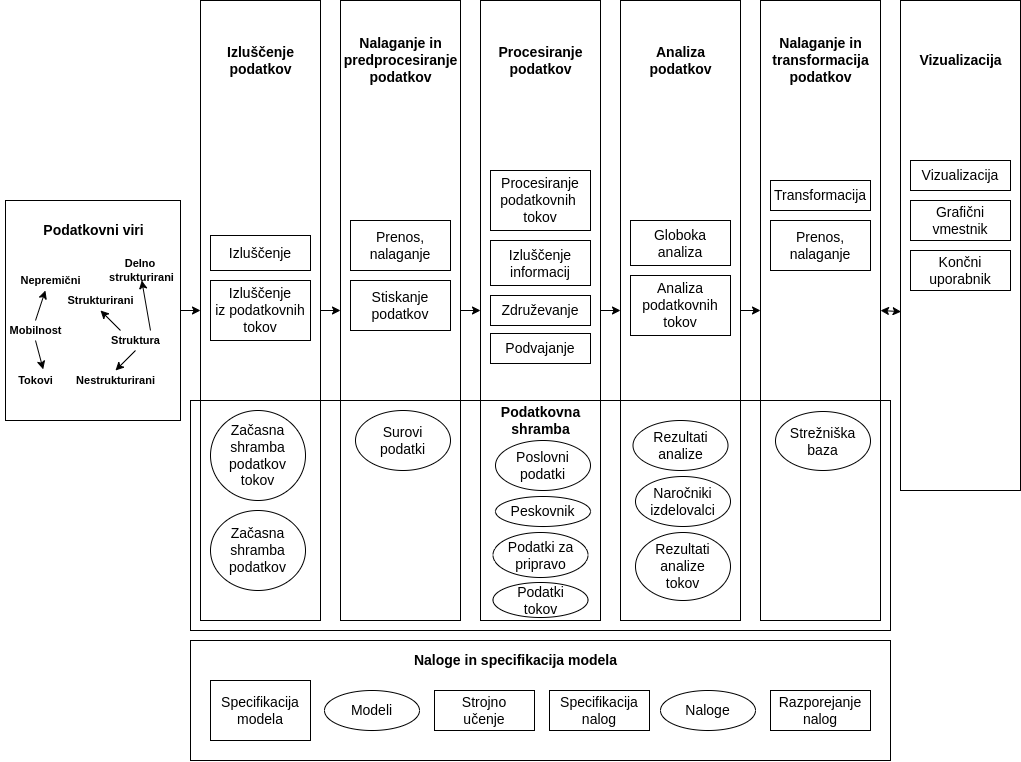
\includegraphics[width=0.99\textwidth]{img/arhitektura/reference.png}
    \caption{Visoko nivojska referenčna arhitektura Big Data aplikacij.
        Podatkovne shrambe so prikazane v elipsah, storitve v kvadratih in
        pot podatkov s puščicami.
        Povzeto po članku~\cite{reference_architecture_classification_technologies}.}
    \label{fig:arch-ref-article}
\end{figure}

\noindent V poglavju~\ref{sec:metodologija} referenčno arhitekturo uporabimo skupaj z
iteracijsko metodo~\cite{iterative_methodology} in
naredimo metodologijo.

\paragraph{Shramba}
Relacijske baze niso primerne za uporabo z nestrukturiranimi podatki.
Prav tako so te baze počasnejše kot NoSQL podatkovne baze,
kar nas omejuje pri analizi big data, saj je hitrost ključnega pomena.
NoSQL podatkovne baze sprostijo strukturo, kar olajša delo z nestrukturiranimi podatki.
Prav tako NoSQL baze omilijo zahteve glede konsistence in
omogočajo večjo dosegljivost in večjo skalabilnost.

V naši metodologiji bomo uporabili Opensearch~\cite{tech_opensearch}, 
ki je odprtokodna veja podatkovne baze Elasticsearch.
Opensearch je NoSQL podatkovna baza, ki omogoča visoko skalabilnost.

\paragraph{Procesiranje podatkov}
Pri delu z big data bomo delali s podatkovnimi tokovi
in potrebujemo orodje, ki je neodvisno od tipa podatkov in omogoča delo z veliko količino podatkov.
Želimo imeti visoko dostopnost in orodje mora ohranjati kvaliteto podatkov.

Uporabili bomo Apache Kafka~\cite{tech_kafka}.
Članek~\cite{iterative_methodology} opisuje Kafkine lastnosti.
Kafka omogoča obdelavo visoke količine podatkov v realnem času.
Podatki so lahko raznoliki in podpira uporabo strukturiranih in nestrukturiranih podatkov.
Kafko garantira, da se podatki ne izgubijo in ne podvojijo.

\section{Metodologije}

\subsection{Metodologije na splošno}
SSKJ metodologijo definira kot \say{skupek metod, ki se uporabljajo pri kakem raziskovanju, mišljenju}~\cite{metodologija_def}.
V računalništvu nam metodologije pomagajo pri odločitvah glede vodenja projektov.
Mnogi programerji jih vsaj okvirno poznajo, kar pospeši uvajanje.

\subsection{Primeri metodologij}
V računalništvu imamo kar nekaj razširjenih metodologij.
Te metodologije nam predpisujejo načine programiranja,
cikle oddajanja programske kode,
načine sodelovanja s stranko in druge dele razvoja.
Spodaj jih opišem samo par~\cite{agile_methodologies}.

\paragraph{Scrum} predpisuje majhne ekipe, ki sledijo predpisanemu šprintu~\cite{scrum_meth}.
Tega pripravi vodja Scruma (\textit{angl. Scrum master})
na podlagi ciljev, ki jih zastavi lastnik produkta (\textit{angl. Product owner}).
Vsak šprint traja predpisano dolžino časa, ponavadi en mesec ali manj.
Na začetku vsakega se izvede načrtovanje, kjer se odgovori na naslednja vprašanja:

\begin{itemize}
    \item Zakaj delamo ta šprint?
    \item Kaj lahko naredimo v tem šprintu?
    \item Kako lahko naredimo naše cilje v tem šprintu?
\end{itemize}

Scrum predpisuje vsakodnevne petnajst minutne sestanke,
kjer se pregleda uspešnost šprinta in uvede spremembe,
če so te potrebne.
Na koncu šprinta se najprej izvede pregled, kjer se pregleda narejeno in 
kaj se bo delalo naprej, 
nato pa se ekipa posvetuje o načinih izboljšave v naslednjem šprintu.
Šprinti se ponavljajo, dokler ni delo končano.

\paragraph{Kanban} uporablja tabla, na kateri so
razporejene naloge glede na stanje~\cite{kanban_meth,kanban_book}.
Tabla je lahko digitalna ali fizična in na njej so naloge ločene
v predpisane stolpce, ki predstavljajo različna stanja nalog, na primer
\textit{čaka}, \textit{v teku}, \textit{v pregledu}, \textit{končano}.
Kanban priporoča omejevanje števila nalog v posameznih stolpcih,
saj delo na več nalogah poslabša efektivnost.
Ne uporablja iteracij, ampak namesto tega meri čas do izdelave
posamezne naloge.

\paragraph{Ekstramno programiranje}
predstavlja skupek praks~\cite{extreme_prog_meth, waterfall_meth}.
En del je opisan v tabeli~\ref{tab:extreme_programming}.
Lahko uporabimo eno, vse ali samo nek del praks.

\begin{table}[H]
    \centering
    \begin{tabularx}{\textwidth}{S S L} 
        Praksa & Angleško & Opis \\ \hline
        
        Igra načrtovanja & Planning game & Stranke se odločijo za obseg
        in časovnico izdaj glede na ocene programerjev.
        Programerji implementirajo samo funkcionalnosti,
        v trenutni iteraciji. \\

        Majhne oddaje & Small releases &
        Sistem se odda v produkcijo že kmalu po začetku dela in
        izboljšave se redno oddajajo. \\

        Testiranje & Tests & Testi se pišejo sproti in
        med implementacijo se preverja,
        da se ni noben test padel. \\

        Programiranje v paru & Pair programming &
        Koda se piše v paru,
        kjer oba uporabljata isti računalnik.

    \end{tabularx}
    \caption{Prakse v extremnem programiranju~\cite{extreme_prog_meth}.}
    \label{tab:extreme_programming}
\end{table}

\paragraph{Slapovno programiranje} je način razvoja~\cite{waterfall_meth},
kjer aplikacije programiramo v predpisanem vrstnem redu.
Na začetku določimo sistemske in aplikacijske zahteve.
Nato se naredi analizo problema,
zasnuje aplikacijo in nato se celotna aplikacija sprogramira.
Na koncu se aplikacijo testira in odda v produkcijo.

V osnovni verziji slapovnega programiranja se ne vračamo nazaj na prejšnji korak,
ampak kasneje so uporabniki te metodologije
sprejemali vračanje nazaj tudi v direktni predhodni korak.

\paragraph{Devops} je združitev razvijalnega in operacijskega dela~\cite{devops_meth}.
Predlaga sprotno in avtomatizirano testiranje, ter sprotno objavljanje v produkcijo.
Želi avtomatizirati tudi operacijske dele,
na primer definicija infrastrukture v kodi.

\subsection{Primerjava tradicionalnih in big data metodologij}

\subsection{Obstoječe big data metodologije}
V članku \cite{iterative_methodology} avtorji predstavijo iterativno metodo za zasnovo arhitekture big data aplikacij.
Njihov algoritem najprej naredi graf vozlišč, kjer vsako predstavlja skupek tehnologij, ki služijo podobni funkciji.
V naslednjih korakih se tehnologije določijo bolj podrobno.
Algoritem za vstop potrebuje analizo zahtev same aplikacije, npr. kako močno konsistenco ali hitro aplikacijo potrebujemo.

Članek~\cite{bigprovision} govori o sistemu, ki ponuja postavitve ogrodja za big data aplikacije.
Govori o razvoju PaaS\todo{Dodaj v slovar kratic.} in kako ponudniki javnih oblakov poskrbijo za infrastrukturo big
data aplikacij.
Opisan sistem lahko z vzorcem vhodnih podatkov in uporabnikovih omejitev virov, sam naredi postavitev
in izbere uporabljene tehnologije.

Članek~\cite{modeling_requirements_big_data} uporabi i* 
(imenovano tudi Grajenje zahtev s poudarkom na agentih \emph{angl. Agent oriented Reqirement Engineering})
in KAOS (\emph{angl. Knowledge acquisition in automated specification}) metodologiji, ki sta implementaciji
GORE (\emph{angl. Goal-oriented requirement engineering})~\cite{goal_oriented_requirements_engineering}.
Metodologija i* se problema loti s poudarkom na agentih, kjer je agent uporabnik
ali storitev z neko določeno nalogo.
Določi cilje in naloge, ter medsebojne odvisnosti med agenti, cilji in nalogami.
Diagram se nato razširi z nalogami, katere je potrebno izpolniti za dosego ciljev.
Metodologija KAOS gradi diagrame s tem ko razlaga \emph{zakaj} nek del potrebujemo.
V članku navede zehteve, ki izhajajo iz 4V in nato kako jih lahko dosežemo.

\section{Metodologija <name pending>}

\subsection{Izbira okolja}

\subsubsection{Uporaba lastne strojne opreme ali oblaka} \label{subsub:oblak-on-prem}

Pri izbiri okolja, se moramo najprej odločiti, ali bomo uporabljali lastne strežnike ali
storitve v oblaku.
Članki~\cite{cloud_computing_issues_challanges,cloud_computing_overview,cloud_computing_today_tomorrow}
predstavijo prednosti in slabosti infrastrukture v oblaku.
V tabeli~\ref{tab:cloud-vs-local-infrastructure} predstavim povzetek primerjave uporabe oblačne in
lastne infrastrukture.

\begin{table}[H]
    \centering
    \begin{tabularx}{\textwidth}{S L L} 
        & Lokalno & Oblak \\
        \hline
        
        Skaliranje & 
        Se lahko prilagodi, 
        ampak stroškov nakupa strežnikov ne povrnemo & 
        Se prilagaja zahtevam \\

        Zasebnost podatkov &
        Podatki ne zapustijo naših strežnikov &
        Podatki se pošiljajo preko omrežja,
        lahko v tuje države,
        na tuje sisteme \\

        Stroški &
        Skupni stroški infrastrukture so višji, 
        stroški posamezne enote procesiranja (npr. ene virtualne naprave), so nižji &
        Skupni stroški infrastrukture so nižji, stroški prenosa podatkov so višji \\
        
        Migracija &
        Migracija med lastnimi strežniki je enostavna &
        Migracija med ponudniki je težka \\

        Dostopnost &
        Ponavadi nižja &
        Ponavadi višja
    \end{tabularx}
    
    \caption{Primerjava infrastrukture v oblaku in lokalno.}
    \label{tab:cloud-vs-local-infrastructure}
\end{table}

\noindent Tabela~\ref*{tab:cloud-vs-local-infrastructure} nam pomaga pri izbiri
okolja.
V naslednjih odsekih bodo naše odločitve odvisne od izbire v tem poglavju.
Takrat se bomo sklicevali na to poglavje in razložili,
na kaj moramo biti pazljivi in kakšne so razlike zaradi odločitve
v tem odseku.

\subsubsection{Virtualizacija}

\subsubsection{Orkestracija}

V tem poglavju se odločamo o izbiri orkestracije ali
ročnega nadziranja aplikacij.
Orodja za orkestracijo skrbijo za nemoteno delovanje aplikacij.
V primerjavi z ročnim upravljanjem orodje za orkestracijo samo skrbi za:
\begin{itemize}
    \item Ugašanje aplikacij, ki so obtičale.
    \item Povezovanjem med aplikacijami.
    \item Zunanjo shrambo.
    \item Skaliranje aplikacij.
\end{itemize}

\noindent Članek~\cite{virtualisation_vs_containerization} primerja uporabo
vsebnikov z uporabo navideznih naprav in primerja
nazlične implementacije orodij za delo z vsebniki.
Moderne aplikacije so sestavljene iz mnogih storitev, zato se za
lažje delo z vsebniki priporoča uporaba orodij za orkestracijo~\cite{container_orchestration}.
Članek~\cite{container_orchestrators_comparison} primerja različne implementacije.
Avtorji priporočajo uporabo Docker Compose ali Docker swarma za testiranje,
ter uporabo Kubernetesa za produkcijo.
Članek~\cite{container_orchestration} primerja implementacije bolj podrobno in
prav tako predlaga Kubernetes,
ampak opozarja na visoko porabo virov v določenih primerih.
Oba članka kot eno izmed možnosti omenjata tudi Apache Mesos,
ki pa ima manjšo bazo uporabnikov in je bolj zahteven za postavitev.
Za primere testiranja predlagamo uporabo orodja Minikube,
ki omogoča enostavno postavitev testne Kubernetes gruče.

Nadaljevanje magistrske naloge se nagiba k uporabi orkestracije,
saj z rastjo arhitekture postane ročno uporavljanje z aplikacijami preveč
zapleteno.
V primeru, da se odločite za ročno upravljanje je potrebno vsak del
arhitekture postaviti po navodilih razvijalca.
Vključitev v magistrsko nalogo je preveč zahtevna,
saj nameščanje vsebuje preveč spremenljivk, na primer 
od operacijskega sistema in tipa podatkovnega sistema.

V primeru, da smo se v poglavju~\ref{subsub:oblak-on-prem} odločili za uporabo oblaka,
nam naš ponudnik pogosto ponuja tudi že uporabo njhovega
orodja za orkestracijo.
V tem primeru, nam v tem koraku ni potrebno narediti ničesar,
drugače pa moramo orodje za orkestracijo postaviti sami.
Če smo izbrali orodje Kubernetes, si lahko pomagamo z orodji \textit{Kubespray} in \textit{kubeadm}
za lažjo postavitiv Kubernetesa.

\subsection{Gradnja arhitekture}

\subsubsection{Analiza zahtev aplikacije}

\subsubsection{Izpolnjevanje zahtev}

\subsection{Dodatki}

\subsubsection{Sprotno objavljanje}

\subsubsection{Testiranje}

\subsubsection{Preverjanje robustnosti}

\listoftodos[TODO]

\cleardoublepage                           % na desni strani
\phantomsection                            % da prav delujejo hiperlinki
\addcontentsline{toc}{section}{\bibname}   % dodajmo v kazalo
\bibliographystyle{fmf-sl}                 % uporabljen stil je v datoteki fmf-sl.bst, na voljo tudi angleška verzija
\bibliography{\literatura}                 % literatura je v datoteki, definirani na začetku
% TeXStudio zmede \ zgoraj, tako da lahko notri napišeš dejansko ime .bib datoteke, če ti
% ne delajo predlogi citatov.

\end{document}
